\documentclass[../main.tex]{subfiles}

\begin{document}

\subsection{Modelo Deep Learning}

Como se puede ver en el apéndice \ref{notebook}, en el entrenamiento del modelo de Deep Learning se consigue un 94,75\% de acierto en el test de validación.

Además, se puede observar en la figura \ref{figure30} el porcentaje de precisión tanto para el dataset de entrenamiento como el de validación, observándose cómo van evolucionando de forma casi idéntica.

En la figura \ref{figure31} se puede ver la matriz de confusión, aunque esta matriz no es representativa del porcentaje de acierto del modelo dado que las clases no están balanceadas, esto provoca que la diagonal no tenga un número similar de aciertos entre clases, pero es debido a la gran diferencia de muestras de unas clases sobre otras.

En la figura \ref{figure32} puede observarse el porcentaje de acierto, exhaustividad y f1-score para cada una de las diferentes clases.

\begin{figure}[h]
\centering 
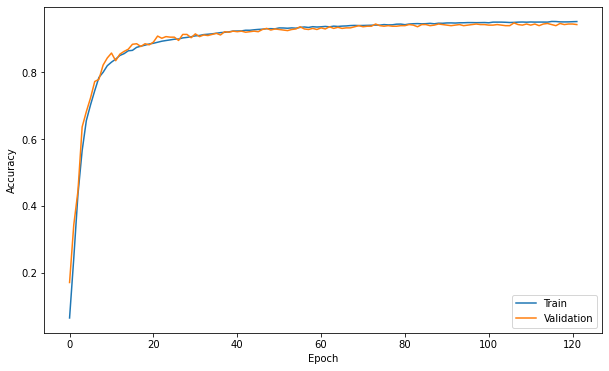
\includegraphics[width=1\textwidth]{notebook/output_9_0.png}
\caption{Evolución de la precisión del dataset de entrenamiento y validación.}
\label{figure30}
\end{figure}

\begin{figure}[h]
\centering 
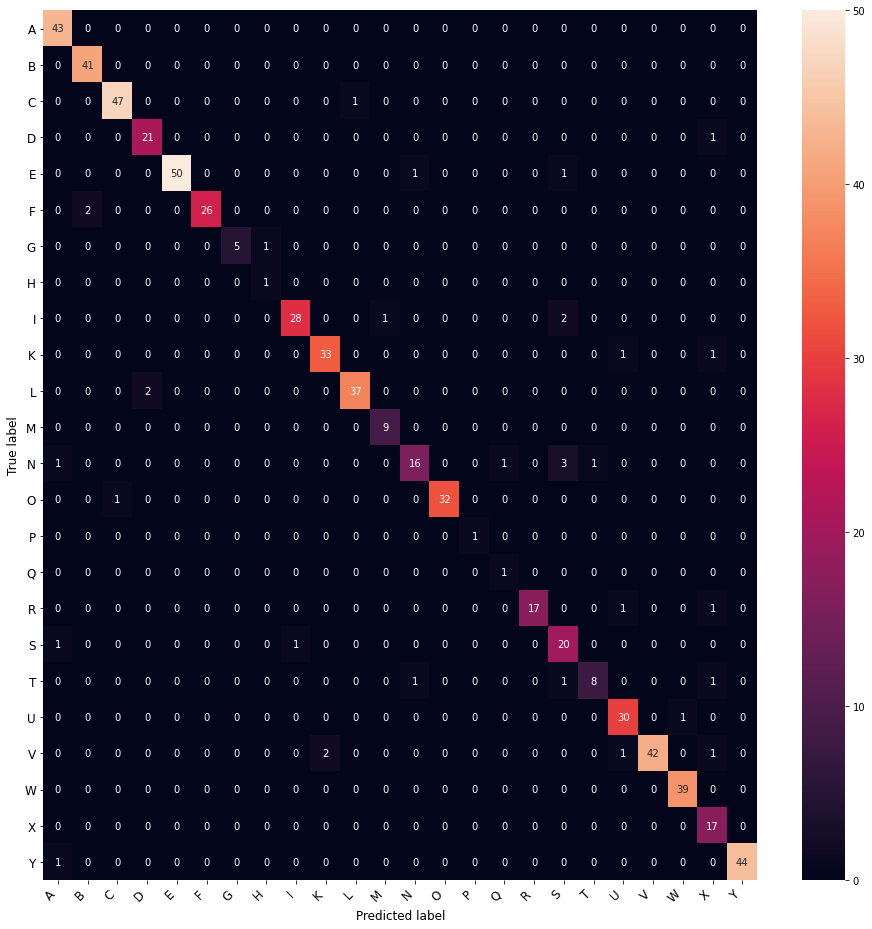
\includegraphics[width=1\textwidth]{notebook/output_10_0.png}
\caption{Matriz de confusión.}
\label{figure31}
\end{figure}

\begin{figure}[h]
\centering 
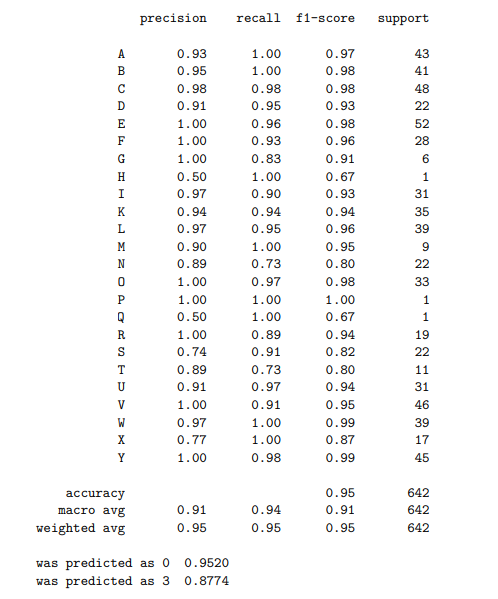
\includegraphics[width=1\textwidth]{images/modelo/recall.PNG}
\caption{Porcentaje de precisión y recall.}
\label{figure32}
\end{figure}

\subsection{iOS App Interpreter American Sign Language}

Para la demostración de resultados, se han utilizado algunos videos de la plataforma \url{http://wwww.youtube.com}. Todas las pruebas se han realizado seleccionando como entrada la cámara del dispositivo, por lo que para el análisis de videos de la plataforma, se proyecta el vídeo en un monitor, de forma que la cámara del dispositivo está enfocada en el monitor y permite realizar el análisis.

También se ha realizado un vídeo para la demostración de resultados del método de funcionamiento Detects words \ref{words}.


\begin{enumerate}
    \item Demo 1 \cite{demo1}: Se utiliza el método de funcionamiento Letter Occurrences. Se consigue acertar en 23 de 24 letras, únicamente fallando la predicción de la letra 'S'. El video original puede encontrarse en \cite{demo1original}.
    \item Demo 2 \cite{demo2}: Se utiliza el método de funcionamiento Letter Occurrences. Se consigue acertar en 22 de 24 letras, fallando en las letras 'N' y 'P'. El vídeo original puede encontrarse en \cite{demo2original}
    \item Demo 3 \cite{demoword}: Se utiliza el método de funcionamiento Detect words y se consigue con éxito acertar todas las letras y distinguir cuando se empieza y acaba una palabra. Este video ha sido realizado para la demostración del TFG.
\end{enumerate}

Para obtener una resultados precisos es necesario que el dispositivo esté situado con un trípode. El entorno en el que se han realizado las pruebas puede verse en \cite{demo1env}.


\end{document}